\documentclass[tikz,border=3pt]{standalone}
% Shared Figure architecture visual system for all four main-text figures.
\usepackage[T1]{fontenc}
\usepackage{charter}
\usepackage[scaled=0.90]{helvet}
\usepackage{amsmath,amssymb}
\renewcommand{\Pr}{\mathbb{P}}
\usepackage{xcolor}
\usepackage{tikz}
\usepackage{pgfplots}
\pgfplotsset{compat=1.18}
\usetikzlibrary{arrows.meta,calc,positioning,fit,decorations.pathreplacing,shapes.geometric,backgrounds}
\definecolor{figNavy}{RGB}{0,63,92}
\definecolor{figBlue}{RGB}{0,101,165}
\definecolor{figSky}{RGB}{226,241,249}
\definecolor{figTeal}{RGB}{0,125,112}
\definecolor{figMint}{RGB}{224,243,239}
\definecolor{figOrange}{RGB}{222,102,35}
\definecolor{figPeach}{RGB}{252,235,224}
\definecolor{figRed}{RGB}{145,43,55}
\definecolor{figInk}{RGB}{35,45,51}
\definecolor{figGray}{RGB}{103,115,123}
\definecolor{figRule}{RGB}{194,202,208}
\definecolor{figPale}{RGB}{248,250,251}
\definecolor{figWhite}{RGB}{255,255,255}
\tikzset{
  figpanel/.style={draw=figRule,line width=0.55pt,rounded corners=2.4pt,fill=figWhite},
  figtag/.style={circle,fill=figBlue,text=figWhite,minimum size=4.3mm,inner sep=0pt,font=\sffamily\bfseries\fontsize{7.5}{8}\selectfont},
  figtitle/.style={font=\sffamily\bfseries\fontsize{8.5}{10}\selectfont,text=figNavy,anchor=west},
  figsubtitle/.style={font=\sffamily\fontsize{6.8}{8}\selectfont,text=figGray,align=left},
  figbody/.style={font=\sffamily\fontsize{7}{8.4}\selectfont,text=figInk,align=center},
  figsmall/.style={font=\sffamily\fontsize{6.2}{7.4}\selectfont,text=figGray,align=center},
  figmath/.style={font=\fontsize{7.4}{8.8}\selectfont,text=figInk,align=center},
  figflow/.style={-{Stealth[length=2.0mm,width=1.4mm]},draw=figBlue,line width=0.85pt},
  figflowgray/.style={-{Stealth[length=1.8mm,width=1.25mm]},draw=figGray,line width=0.75pt},
  figfloworange/.style={-{Stealth[length=2.0mm,width=1.4mm]},draw=figOrange,line width=0.85pt},
  figbluebox/.style={draw=figBlue,line width=0.65pt,fill=figSky,rounded corners=2.2pt},
  figorangebox/.style={draw=figOrange,line width=0.65pt,fill=figPeach,rounded corners=2.2pt},
  figtealbox/.style={draw=figTeal,line width=0.65pt,fill=figMint,rounded corners=2.2pt},
  figgraybox/.style={draw=figRule,line width=0.6pt,fill=figPale,rounded corners=2.2pt},
}
\newcommand{\PanelHeading}[4]{%
  \node[figtag] at (#1,#2) {#3};%
  \node[figtitle] at ({#1+0.32},#2) {#4};%
}


\begin{document}
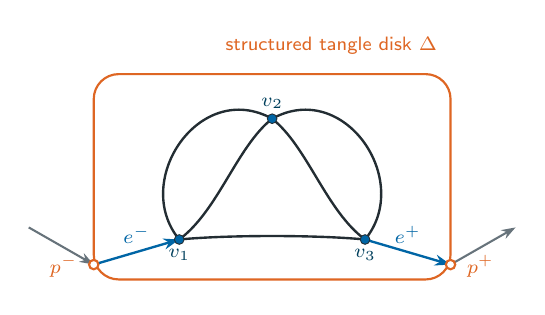
\begin{tikzpicture}[x=1.18cm,y=1.18cm]
  \coordinate (v1) at (-1.00,-0.35);
  \coordinate (v2) at ( 0.00, 0.95);
  \coordinate (v3) at ( 1.00,-0.35);
  \coordinate (pm) at (-1.92,-0.62);
  \coordinate (pp) at ( 1.92,-0.62);
  \coordinate (xm) at (-2.62,-0.22);
  \coordinate (xp) at ( 2.62,-0.22);

  % Structured tangle disk; its label sits above the boundary and strands.
  \draw[draw=figOrange,line width=0.78pt,rounded corners=9pt]
    (-1.92,-0.78) rectangle (1.92,1.43);
  \node[
    font=\sffamily\fontsize{7.0}{8.2}\selectfont,
    text=figOrange,
    anchor=south east
  ] at (1.88,1.54) {structured tangle disk $\Delta$};

  % The two joining edges and their initial segments inside the disk.
  \draw[figflowgray] (xm) -- (pm);
  \draw[figflowgray] (pp) -- (xp);
  \draw[figflow] (pm) -- (v1);
  \draw[figflow] (v3) -- (pp);

  % Five internal edges: multiplicities 2,2,1.
  \draw[draw=figInk,line width=0.86pt,line cap=round]
    (v1) .. controls (-1.52,0.28) and (-0.78,1.38) .. (v2);
  \draw[draw=figInk,line width=0.86pt,line cap=round]
    (v1) .. controls (-0.58,-0.04) and (-0.38,0.65) .. (v2);
  \draw[draw=figInk,line width=0.86pt,line cap=round]
    (v2) .. controls (0.38,0.65) and (0.58,-0.04) .. (v3);
  \draw[draw=figInk,line width=0.86pt,line cap=round]
    (v2) .. controls (0.78,1.38) and (1.52,0.28) .. (v3);
  \draw[draw=figInk,line width=0.86pt,line cap=round]
    (v3) .. controls (0.48,-0.30) and (-0.48,-0.30) .. (v1);

  % Crossing vertices and the two boundary cut points.
  \foreach \p in {v1,v2,v3}
    \filldraw[fill=figBlue,draw=figInk,line width=0.32pt]
      (\p) circle (1.75pt);
  \filldraw[fill=figWhite,draw=figOrange,line width=0.78pt]
    (pm) circle (1.70pt);
  \filldraw[fill=figWhite,draw=figOrange,line width=0.78pt]
    (pp) circle (1.70pt);

  % Minimal mathematical labels.
  \node[font=\fontsize{7.0}{8.2}\selectfont,text=figNavy,anchor=north]
    at (v1) {$v_1$};
  \node[font=\fontsize{7.0}{8.2}\selectfont,text=figNavy,anchor=south]
    at (v2) {$v_2$};
  \node[font=\fontsize{7.0}{8.2}\selectfont,text=figNavy,anchor=north]
    at (v3) {$v_3$};
  \node[font=\fontsize{6.8}{8.0}\selectfont,text=figOrange,anchor=east]
    at (-1.99,-0.64) {$p^-$};
  \node[font=\fontsize{6.8}{8.0}\selectfont,text=figOrange,anchor=west]
    at (1.99,-0.64) {$p^+$};
  \node[font=\fontsize{7.0}{8.2}\selectfont,text=figBlue]
    at (-1.46,-0.30) {$e^-$};
  \node[font=\fontsize{7.0}{8.2}\selectfont,text=figBlue]
    at (1.46,-0.30) {$e^+$};
\end{tikzpicture}
\end{document}
